\section{Data Warehouse}\label{sec:data_warehouse}

\begin{figure*}[t]
\centering
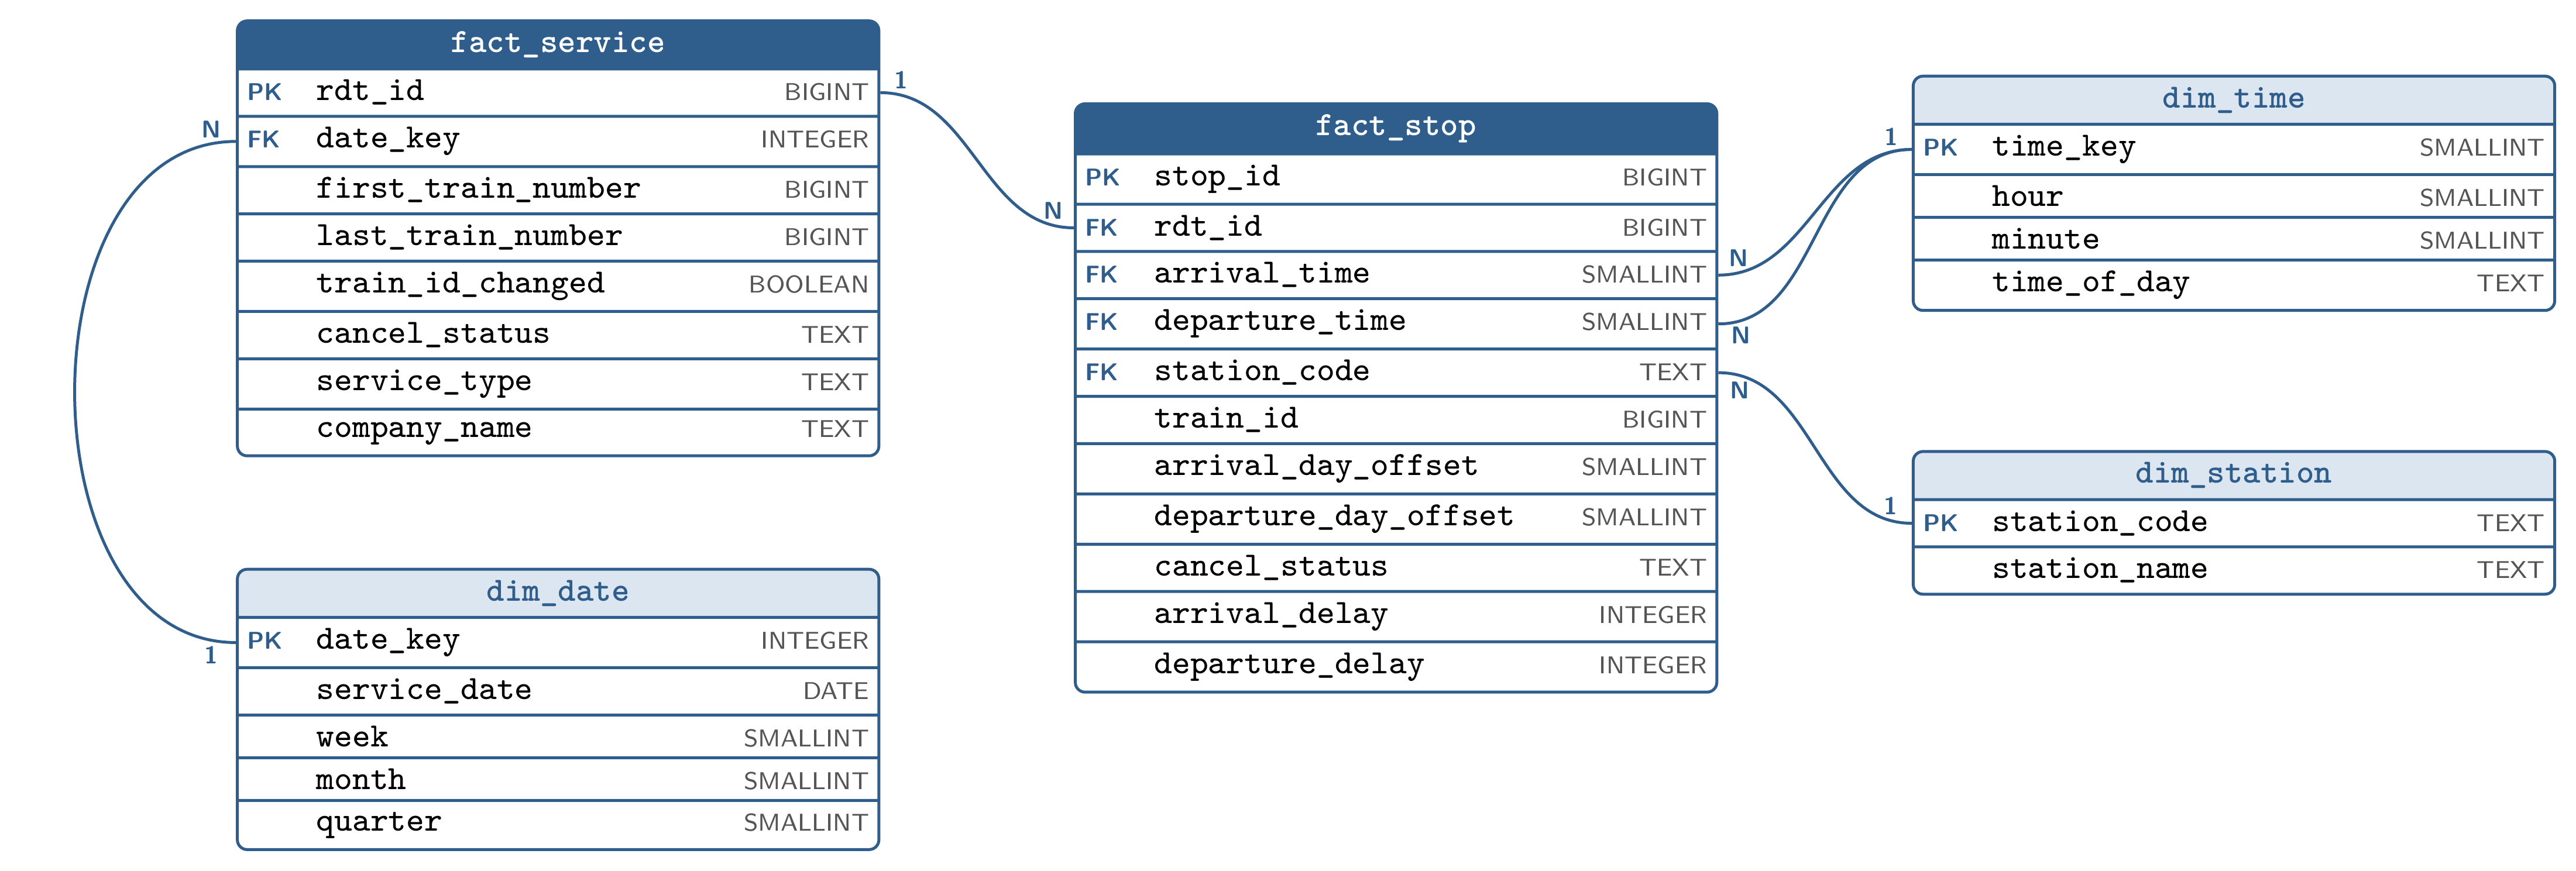
\includegraphics[width=\textwidth]{figures/schema.png}
\caption{Schema of the data warehouse. Dark headers are fact tables and light headers are dimension tables. Each line joins a foreign key (N) to the primary key it references (1).}
\Description{Entity-relationship diagram of the warehouse. fact\_service references dim\_date through date\_key. fact\_stop references fact\_service through rdt\_id, dim\_time through arrival\_time and departure\_time, and dim\_station through station\_code.}
\label{fig:schema}
\end{figure*}

The creation of the database schema seen in Figure~\ref{fig:schema} was informed by the aforementioned EDA and domain knowledge. Given that the schema utilizes 2 fact tables, 
\textit{fact\_service} and \textit{fact\_stop}, it is a galaxy schema by definition \cite{g4g-galaxy}, though it retains the principles of a star schema design as well. The decision 
to use two fact tables was driven the difference in granularity between the two tables, as the service table corresponds to a train's entire trip, while the stop 
table represents one arrival or departure within a trip. 

The service table contains an RDT ID as its primary key, along with a date key as its foreign key. The service table also contains fields that denote 
whether or not its train changed midway, whether the service was cancelled (and to what degree), its service type, and the name of the company administering the service.
The stop table contains a stop ID as its primary key, while its foreign keys consist of the RDT id of its corresponding service, the arrival and derparture times, and
the station code. Additionally, it contains information regarding train ID, arrival and departure day offset, cancellation status, and arrival and departure delays. The two
fact tables are connected by a one-to-many relationship from the stop table to the service table, as one train service contains multiple stops itself.

To provide further context to the existing fact tables, three dimensional tables were created, \textit{dim\_time}, \textit{dim\_station}, and \textit{dim\_date}. 
The time and station dimensions connect to the stop table, while the date dimension connects to the service table. The time dimension's hierarchy focuses on drilling down 
from a general time of day (morning, afternoon, evening) to the hour, and then by the minute. It has two instances of a one-to-many relationship with the stop table, as the 
2 relationships pertain to the arrival and departure times to and from a stop. The station dimension contains the station's code and its name, and maintains a one-to-many 
relationship with the stop table as well since one station houses multiple instances of a train stopping there. Lastly, the date dimension connects to the service table, and its 
hierarchy focuses on drilling down from the quarter, to month, to week, and then to the service's actual date. Similar to the other dimension tables, it has a one-to-many 
relationship with its corresponding fact table, as every day sees multiple train services.

One of the challenges that we encountered in the creation of the data warehouse was the initial difficulty in understanding the relationships between the columns. It took 
a collective effort backed by domain research on the Dutch railway system to break down the meaning of terms such as \textit{service}, \textit{stop}, \textit{RDT}, and 
\textit{cancellation} within the context of the dataset. Another challenge initially faced concerned the size of the dataset, which made it difficult and extremely time-consuming 
to open. In order to circumvent this, \textit{OpenRefine} was used to initially view the data, which was then codensed into an Apache Parquet file that significantly reduced its size. 
Afterwards, the data became more manageable to handle, especially for tasks such as the EDA performed earlier that provided further insight into the dataset that would inform our
decision-making. It is also worth noting that the original CSV file of the dataset contained 3 columns named \textit{Stop: Platform change}, \textit{Stop: Planned 
platform}, and \textit{Stop: Arrival platform}  that focus on the platform where a train stopped. However, this is not as much of a measure of efficiency compared to time, 
station, and date. Additionally, these 3 columns are not listed in the DuckDB documentation's list of columnns in the dataset, so they were ommitted 
from the creation of the database schema. 
